% Appendix
\chapter{USING OUR CUSTOM ENVIRONMENT FOR RL EXPERIMENTATION}
% \setstretch{1.0}
% \inputminted[linenos,tabsize=2,breaklines]{csharp}{clean_code_fucnt.cs}

In this chapter we discuss how to set up Unity and the resources required for the running project. Unity is a free for personal use game development engine, and it UnityHub can be downloaded from  \href{https://store.unity.com/#plans-individual}{https://store.unity.com/#plans-individual}. After installing UnityHub, install Unity version 2019.4.25f1.

Clone the project repository into the system from \href{https://github.com/MaheshBharadwaj/UnityRacer}{https://github.com/MaheshBharadwaj/UnityRacer}.
Open the cloned project in UnityHub using the installed version of Unity. Click on Window $\rightarrow$ Package Manager $\rightarrow$ Unity Registry, search for MLagents version 2.1.0 and install. Finally, install the MLAgents python package using pip or conda from \href{https://pypi.org/project/mlagents/}{https://pypi.org/project/mlagents/}.

Once you have completed these steps, you will be able to explore the environments we have created. You will also be able to access the prefabs created by us in Assets $\rightarrow$ Prefabs. The 3 prefabs as seen in figure \ref{fig:prefabs} are the building blocks of all the tracks that we have created. 

Click on File $\rightarrow$ New Scene and use the track prefabs shown in \ref{fig:prefabs} to create a new track. Ensure the track is created withing a game object and drag and drop the TrackCheckpoints.cs script onto the game object. After creating the layout of the track, drag and drop the checkpoint prefab onto the track. Copy and paste the checkpoints one after another across the track. Ensure that the checkpoints are in sequential order and are roughly equidistant from each other to ensure optimal performance. We also recommend increasing the density of the number of checkpoints during sharp turns to improve the agent performance.
 
\begin{figure}[H]
    \centering
    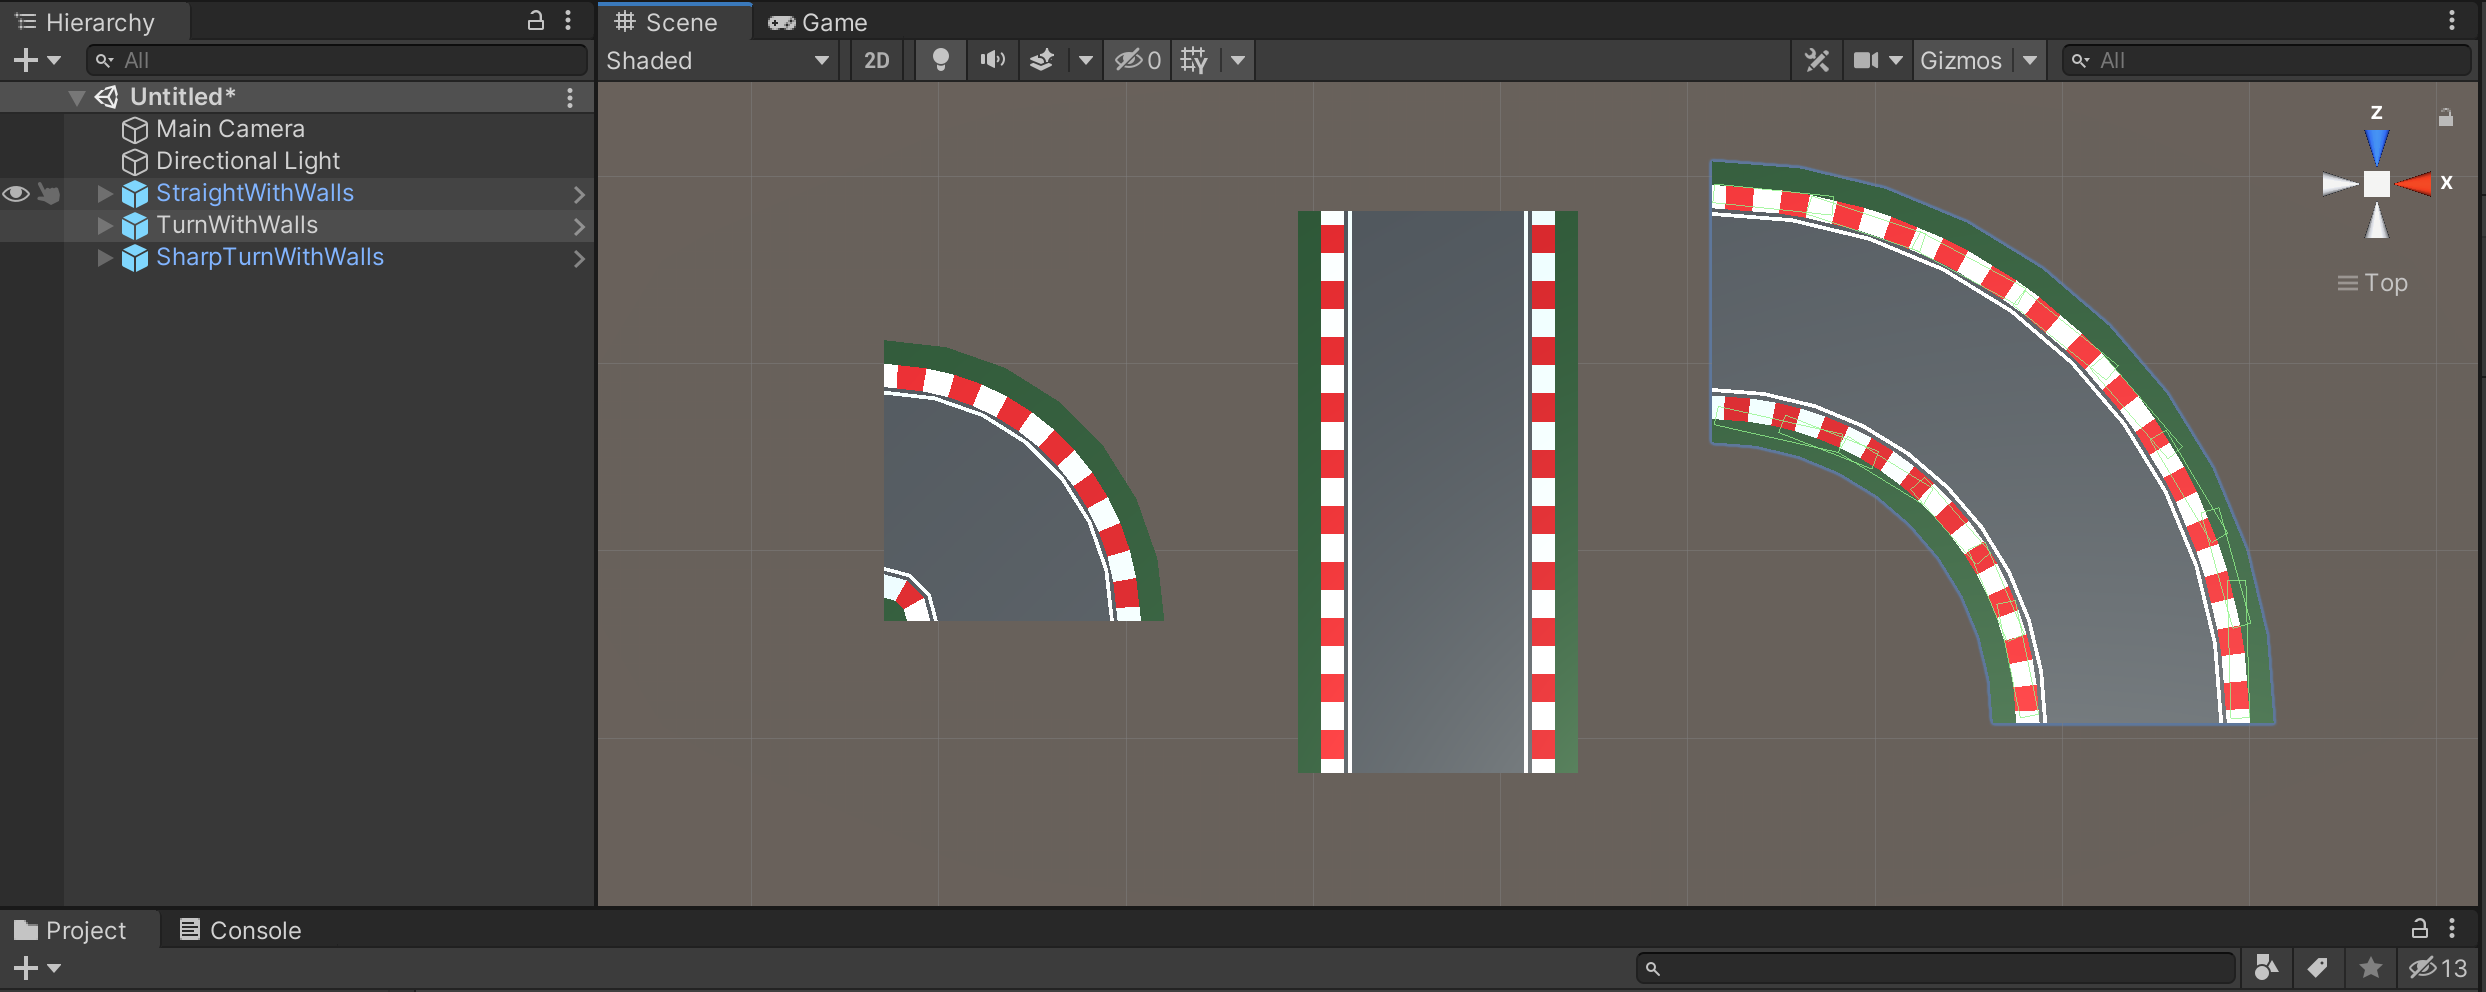
\includegraphics[width=1.0\textwidth]{images/Appendix_scene_prefabs.png}
    \caption{Prefabs L-R: Sharp Turn, Straight, Sweeping Turn}
    \label{fig:prefabs}
\end{figure}

Once the checkpoints are placed, you can drag and drop the `player' from the prefabs folder onto the track right before the first checkpoint. Adjust the position of the player appropriately. The player prefab, comes with numerous features associated with it, on clicking the player component in Unity, check the inspector panel on the right side of the console to setup the agent features.

There are two types of adversarial training. To enable the observation adversary, click on the game object in which the track is present. This will open the inspector panel on the right. In this panel check the `Is Adversarial Training' box, as seen in \ref{fig:AT-Console}
To enable action adversary, click on the player, and in the inspector panel, in the `Car Driver AI' section, set the `Action Adversary' value as a number between 0 and 1.
Shown in \ref{fig:AAT-Console}

\begin{figure}[H]
    \centering
    \begin{minipage}[b]{0.45\textwidth}
    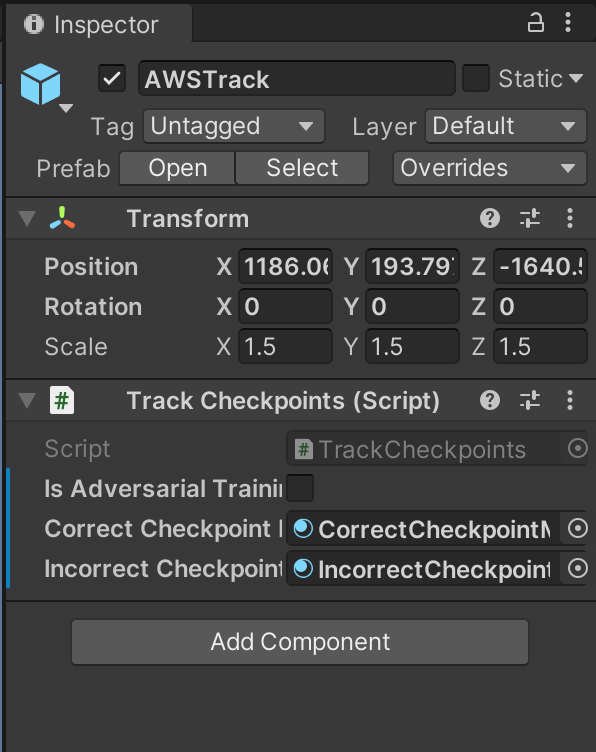
\includegraphics[width=\textwidth]{images/AT-console.png}
    \caption{Enabling AT}
    \label{fig:AT-Console}
  \end{minipage}
  \hfill
  \begin{minipage}[b]{0.45\textwidth}
    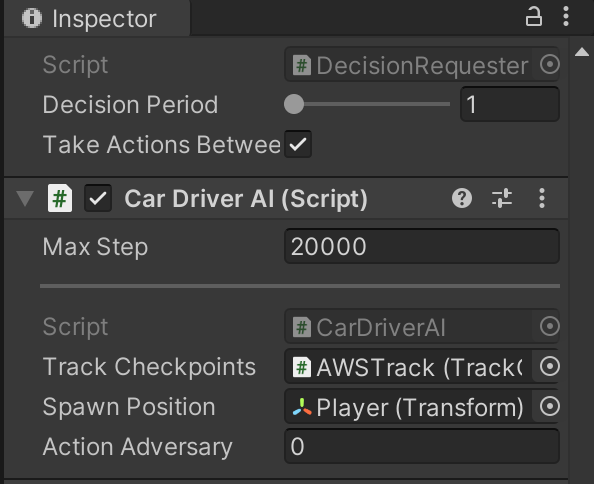
\includegraphics[width=\textwidth]{images/AAT-console.png}
    \caption{Enabling AAT}
    \label{fig:AAT-Console}
  \end{minipage}
\end{figure}


Before training, open the config file named common\_config\_ppo.yaml and set the required parameters in the file. After setting the hyperparameters, use the `mlagents-learn' command while specifying the config file and the run-id in a terminal to start the training process. After running the commamnd open the Unity environment and click on the `Play' button. Once training is finished, the model will be available as a .onnx file in the results folder within a folder having the same name as the run-id.

To use transfer learning open the config file named TL\_config.yaml and set the hyperparameters. Make sure to set the initialize\_from field with the run-id of the source task to enable transfer learning. After setting up the config file. Use the same command `mlagents learn' and specify the TL\_config file to start training process.

To test the models, click on the player component and navigate to the Behaviour parameters in the inspect panel of the console. There you can select a .onnx file model. On doing so, the player will use this model file to travel around the track.

To analyze the results go to the project folder and run the command `tensorboard --logdir results --port 6006'. After running the command open http://localhost:6006/ in a browser. This will allow you to visualize the results of the various models you have trained, on your browser. 



% \begin{itemize}
%     \item Install unity
%     \item Install ML Agents
%     \item Clone the repo for Racerdeep
%     \item Open the prefabs made for sharp turn, turn and straight
%     \item Creating a new track in a new scene
%     \item Adding behaviour parameters and setting up the scripts for the agent training.
%     \item using adversarial training.
%     \item How to config the PPO algorithim and start training
%     \item How to analyse the results
% \end{itemize}

